%% Creator: Inkscape inkscape 0.92.2, www.inkscape.org
%% PDF/EPS/PS + LaTeX output extension by Johan Engelen, 2010
%% Accompanies image file 'regimes1.eps' (pdf, eps, ps)
%%
%% To include the image in your LaTeX document, write
%%   \input{<filename>.pdf_tex}
%%  instead of
%%   \includegraphics{<filename>.pdf}
%% To scale the image, write
%%   \def\svgwidth{<desired width>}
%%   \input{<filename>.pdf_tex}
%%  instead of
%%   \includegraphics[width=<desired width>]{<filename>.pdf}
%%
%% Images with a different path to the parent latex file can
%% be accessed with the `import' package (which may need to be
%% installed) using
%%   \usepackage{import}
%% in the preamble, and then including the image with
%%   \import{<path to file>}{<filename>.pdf_tex}
%% Alternatively, one can specify
%%   \graphicspath{{<path to file>/}}
%% 
%% For more information, please see info/svg-inkscape on CTAN:
%%   http://tug.ctan.org/tex-archive/info/svg-inkscape
%%
\begingroup%
  \makeatletter%
  \providecommand\color[2][]{%
    \errmessage{(Inkscape) Color is used for the text in Inkscape, but the package 'color.sty' is not loaded}%
    \renewcommand\color[2][]{}%
  }%
  \providecommand\transparent[1]{%
    \errmessage{(Inkscape) Transparency is used (non-zero) for the text in Inkscape, but the package 'transparent.sty' is not loaded}%
    \renewcommand\transparent[1]{}%
  }%
  \providecommand\rotatebox[2]{#2}%
  \ifx\svgwidth\undefined%
    \setlength{\unitlength}{556.9991112bp}%
    \ifx\svgscale\undefined%
      \relax%
    \else%
      \setlength{\unitlength}{\unitlength * \real{\svgscale}}%
    \fi%
  \else%
    \setlength{\unitlength}{\svgwidth}%
  \fi%
  \global\let\svgwidth\undefined%
  \global\let\svgscale\undefined%
  \makeatother%
  \begin{picture}(1,0.59015529)%
    \put(0,0){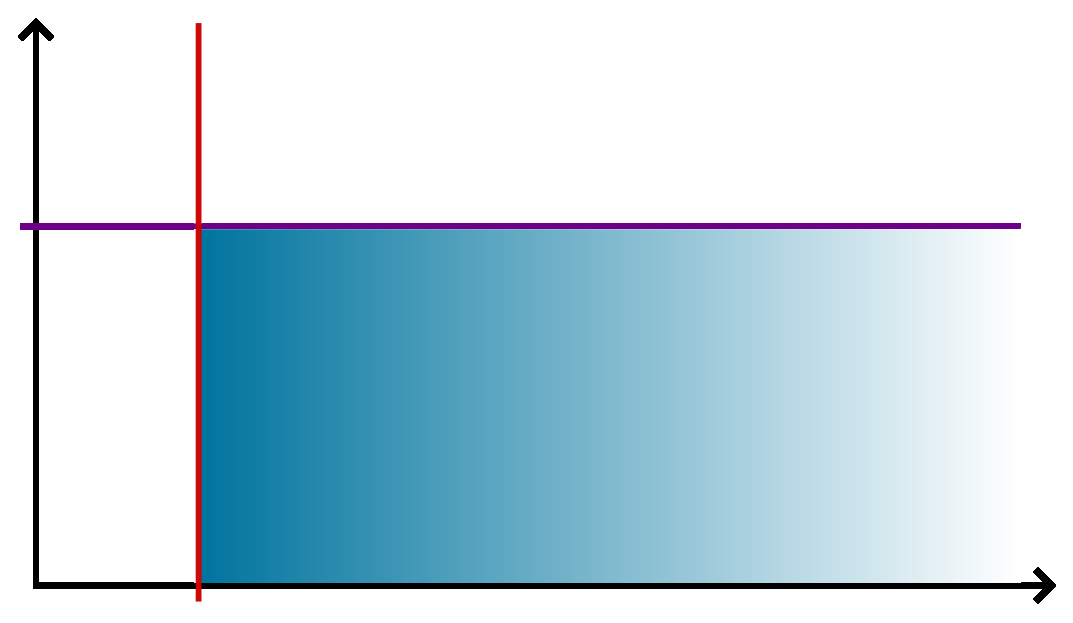
\includegraphics[width=\unitlength]{images_2ddl/regimes1.eps}}%
    \put(0.02561396,0.28811823){\color[rgb]{0,0,0}\makebox(0,0)[lb]{\smash{}}}%
    \put(0.066009,0.05921302){\color[rgb]{0,0,0}\makebox(0,0)[lb]{\smash{}}}%
    \put(-0.01,0.0){\color[rgb]{0,0,0}\makebox(0,0)[lb]{\smash{0}}}%
    \put(-0.0384028,0.35794642){\color[rgb]{0,0,0}\makebox(0,0)[lb]{\smash{0.1}}}%
    \put(0.170346148,-0.02){\color[rgb]{0,0,0}\makebox(0,0)[lb]{\smash{1}}}%
    \put(0.095137172,0.25955463){\color[rgb]{0.8,0,0}\makebox(0,0)[b]{\smash{PAS}}}%
    \put(0.095137172,0.20955463){\color[rgb]{0.8,0,0}\makebox(0,0)[b]{\smash{DE}}}%
    \put(0.095137172,0.15955463){\color[rgb]{0.8,0,0}\makebox(0,0)[b]{\smash{SAUT}}}%
    \put(0.350802717,0.23077807){\color[rgb]{0,0,0.01176471}\makebox(0,0)[b]{\smash{SAUT AVEC PEU}}}%
    \put(0.350802717,0.18077807){\color[rgb]{0,0,0.01176471}\makebox(0,0)[b]{\smash{DE VIBRATIONS}}}%
    \put(0.75539718,0.20955463){\color[rgb]{0,0,0.02745098}\makebox(0,0)[b]{\smash{SAUT  EFFICACE À 50\%}}}%
    \put(0.22758915,0.44969837){\color[rgb]{0,0,0}\makebox(0,0)[lb]{\smash{}}}%
    \put(0.58988013,0.43773024){\color[rgb]{0.43137255,0,0.53333333}\makebox(0,0)[b]{\smash{NON LINÉARITÉ GÉOMÉTRIQUE}}}%
    \put(0.0,0.59741848){\color[rgb]{0,0,0}\makebox(0,0)[lb]{\smash{$\dfrac{F}{kR}$}}}%
    \put(0.96816481,0.05921302){\color[rgb]{0,0,0}\makebox(0,0)[lb]{\smash{}}}%
    \put(1.01,0.01016188){\color[rgb]{0,0,0}\makebox(0,0)[lb]{\smash{$\dfrac{F}{m_r g}$}}}%
  \end{picture}%
\endgroup%
